\graphicspath{{png/}}

\section{Демонстрация работы программы}

Плоское затенение. Даже при большой степени аппроксимации видны полосы.

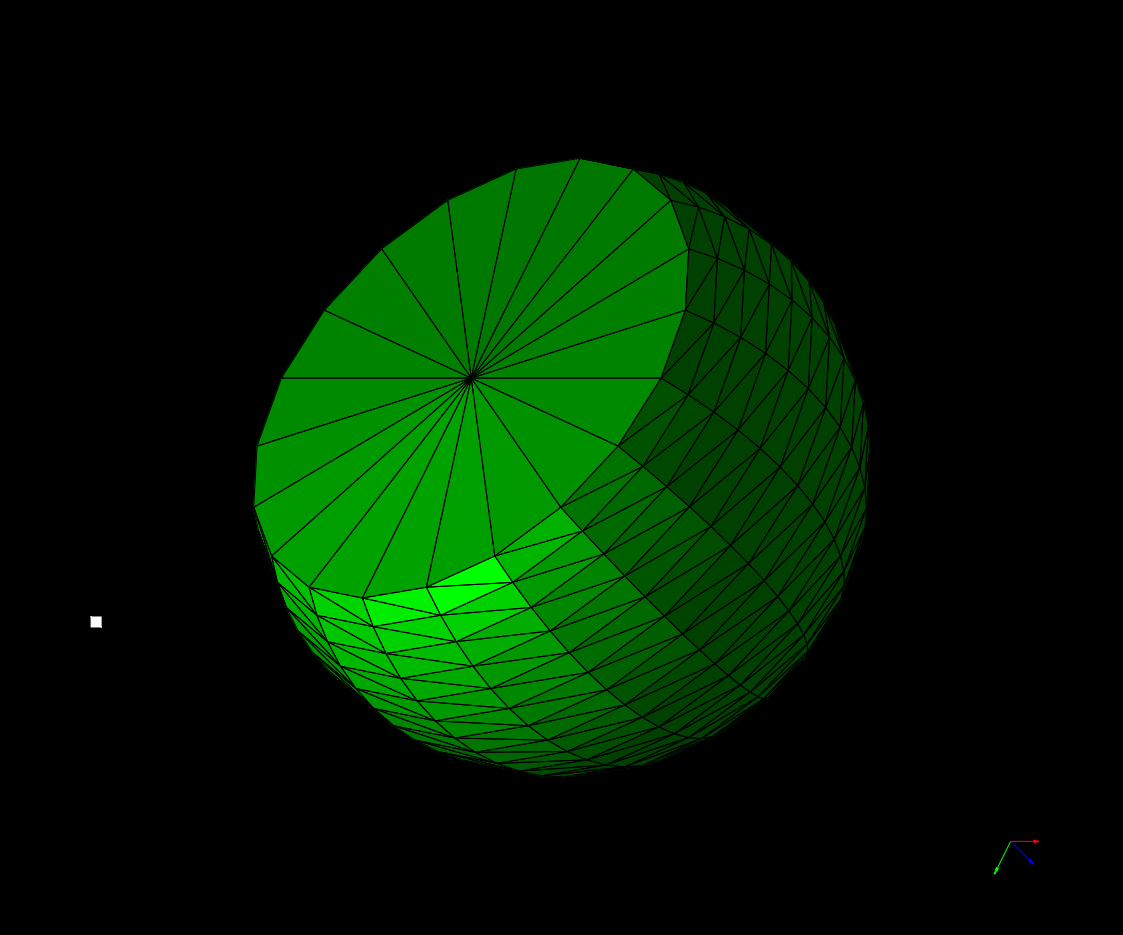
\includegraphics[scale=0.2]{img1}
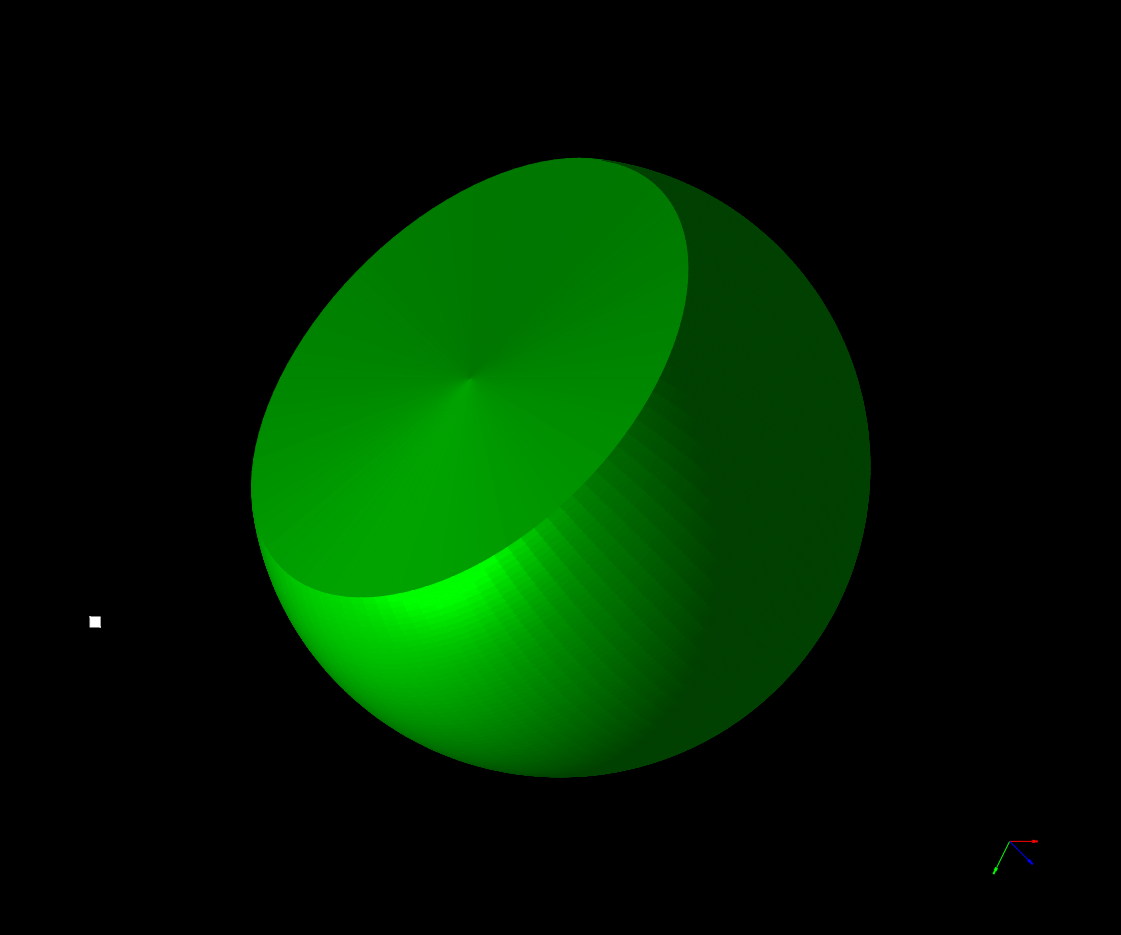
\includegraphics[scale=0.2]{img2}

Затенение Гуро. Предусмотрена возможность отрисовки падающего и отраженно луча для полигона.

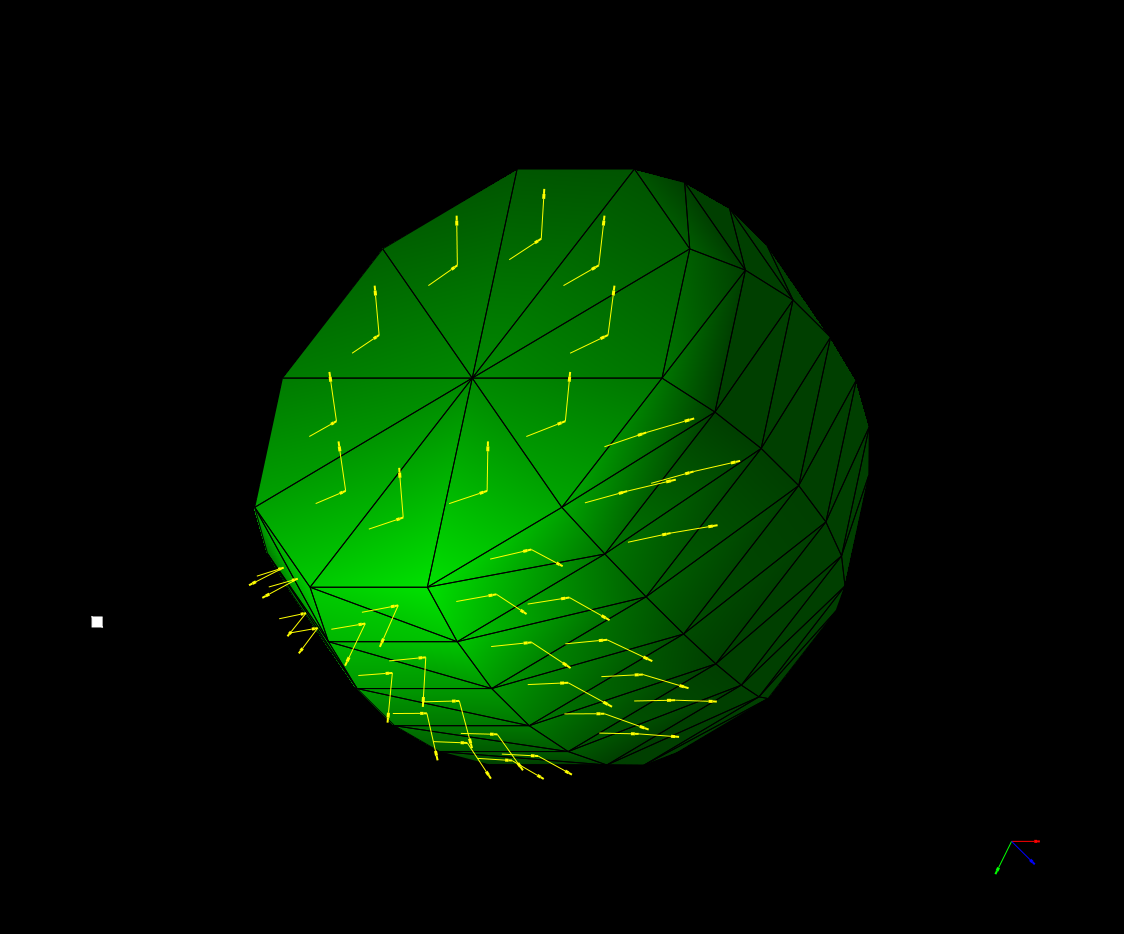
\includegraphics[scale=0.2]{img3}
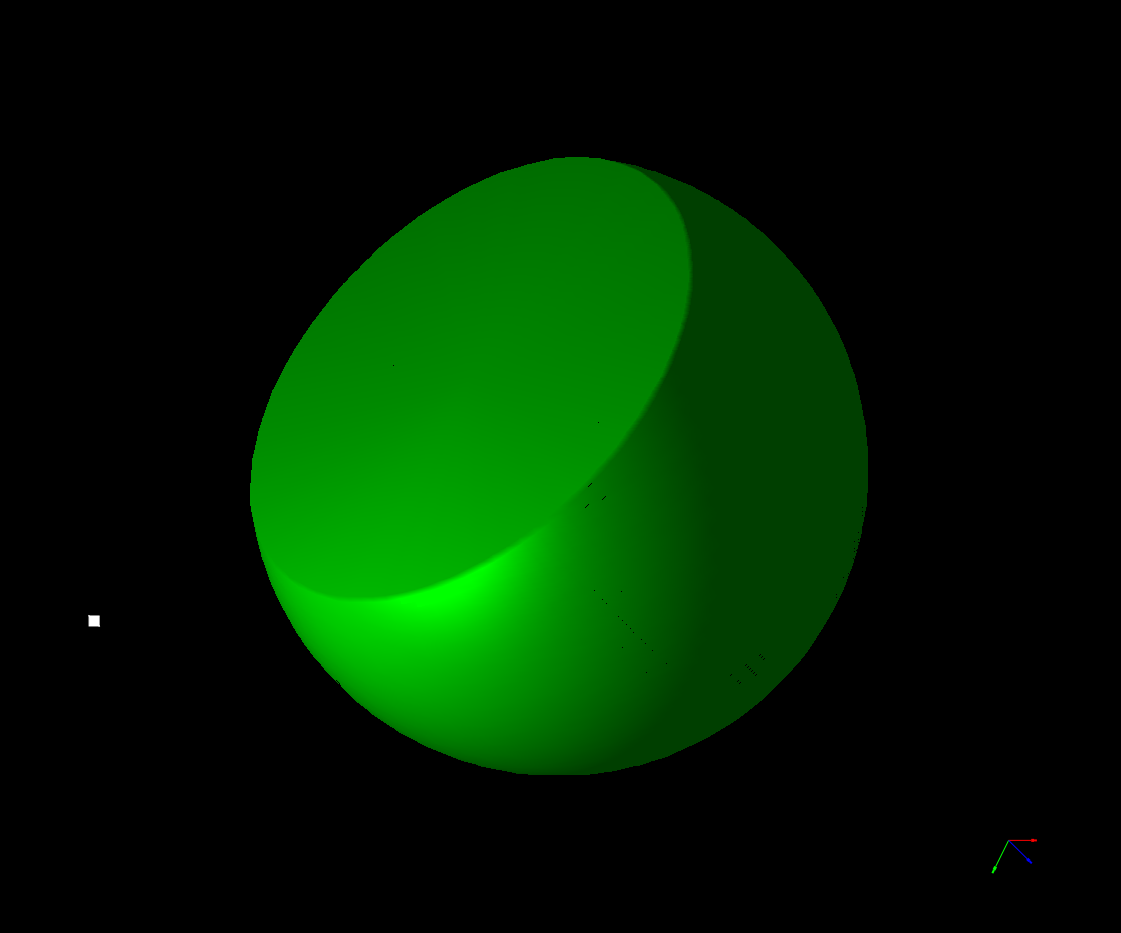
\includegraphics[scale=0.2]{img4}
\pagebreak

Рассеянная и зеркальная состовляющая освещения. Слева только рассенянная, справа обе состовляющие.

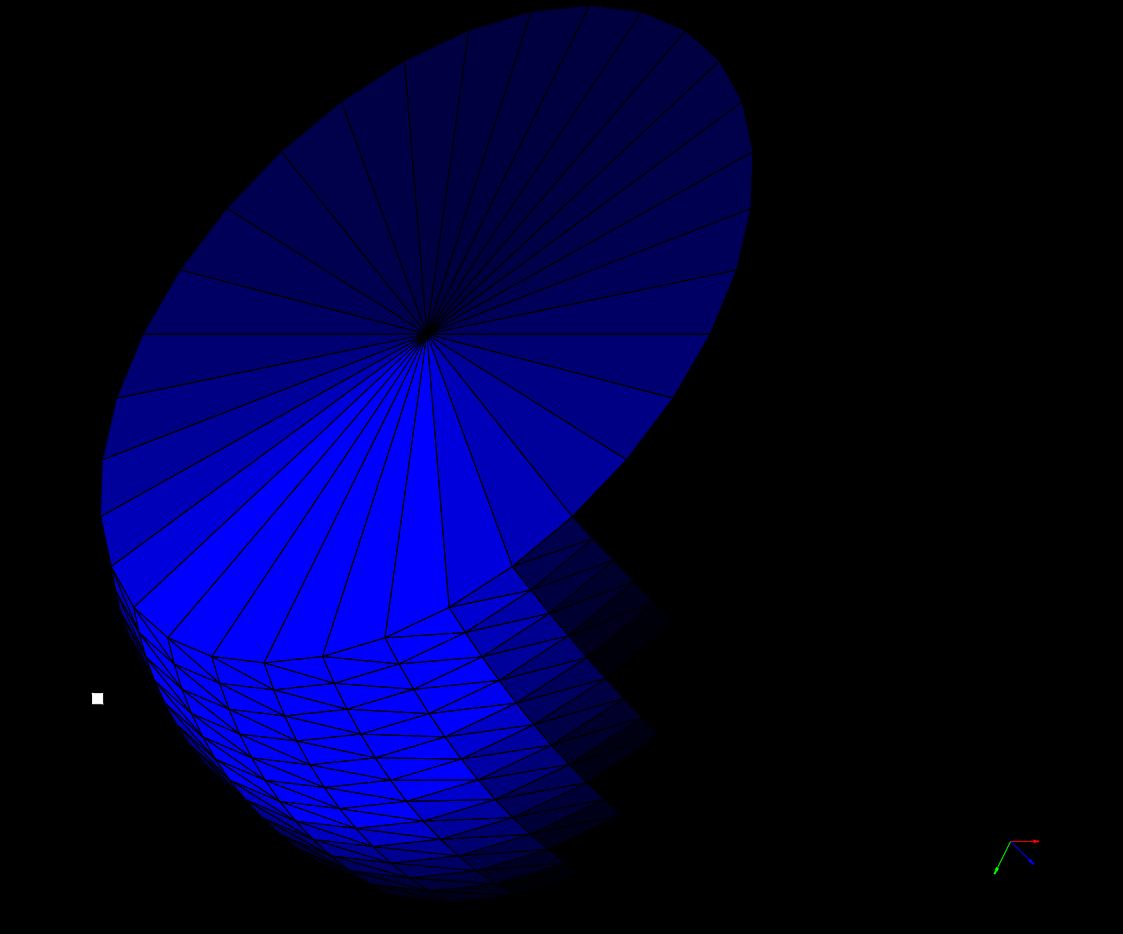
\includegraphics[scale=0.2]{img5}
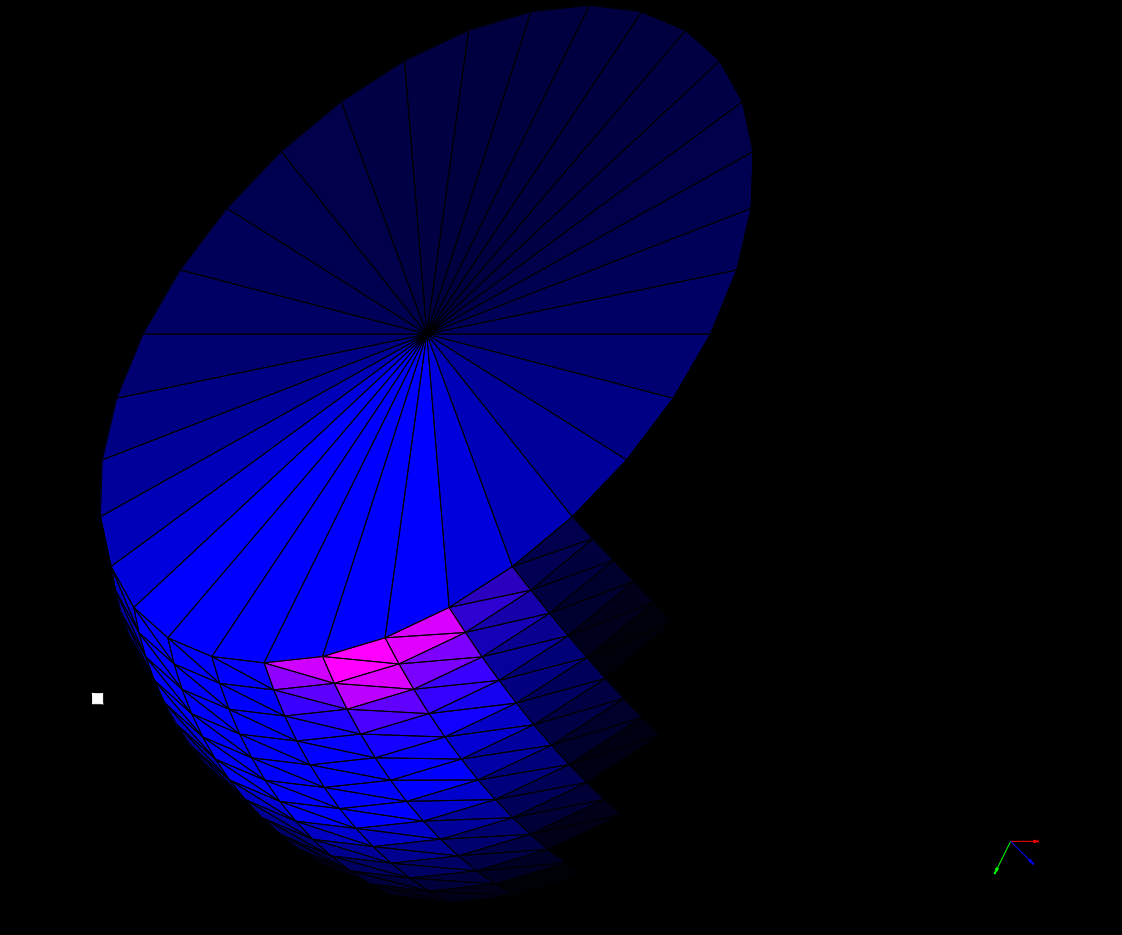
\includegraphics[scale=0.2]{img6}
\pagebreak
